% SHIFT -- JSS manuscript (single-file source; references in references.bib).
% Every number in this file is generated by analysis/*.py from results/raw/** (see Data Availability).
\documentclass[a4paper,fleqn]{cas-sc}
\usepackage[T1]{fontenc}
\usepackage[authoryear,round]{natbib}
\usepackage{amsmath,amsfonts,amssymb,amsthm,algorithm,algpseudocode,array,textcomp,url,graphicx}
\usepackage{tikz,pgfplots,listings,booktabs,xcolor,multirow,needspace}
\usepackage{placeins}
\hypersetup{hypertexnames=false,hidelinks}
\pgfplotsset{compat=1.17}
\usetikzlibrary{positioning,arrows.meta,fit,backgrounds,calc,shapes.misc,patterns}
\newcommand{\tool}{\textsc{Shift}}
\newcommand{\code}[1]{\texttt{\detokenize{#1}}}
\newcommand{\pending}[1]{\textcolor{red}{[#1]}}
\newcommand{\lab}[1]{\textsf{#1}}
\newtheorem{definition}{Definition}
\newtheorem{proposition}{Proposition}
\lstset{basicstyle=\ttfamily\footnotesize,breaklines=true,columns=fullflexible,frame=single,xleftmargin=1em}
\makeatletter
\providecommand\insert@pcolumn{\insert@column}
\providecommand\ext@lstlisting{lol}
\makeatother
\renewcommand{\topfraction}{.95}
\renewcommand{\bottomfraction}{.85}
\renewcommand{\textfraction}{.05}
\renewcommand{\floatpagefraction}{.75}
\setcounter{topnumber}{3}
\setcounter{bottomnumber}{2}
\setcounter{totalnumber}{4}
% BEGIN:results-macros
\newcommand{\exOracleCalls}{8}
\newcommand{\nAgentValid}{1{,}209}
\newcommand{\nCandidates}{1{,}676}
\newcommand{\nGoldValid}{252}
\newcommand{\nGpuHours}{11.6}
\newcommand{\nGpuHoursNarval}{4.3}
\newcommand{\nGpuHoursRorqual}{7.3}
\newcommand{\nGpuJobs}{27}
\newcommand{\nLlmGenerations}{25{,}245}
\newcommand{\nNotValid}{2}
\newcommand{\nOtherStatus}{0}
\newcommand{\nUnits}{3{,}731}
\newcommand{\nValidPatches}{1{,}461}
\newcommand{\rqfourCallsMedian}{3}
\newcommand{\rqfourCallsPninety}{11}
\newcommand{\rqfourCoupled}{40}
\newcommand{\rqfourExhLarger}{0}
\newcommand{\rqfourExhMatch}{99.8\%}
\newcommand{\rqfourExhN}{1{,}397}
\newcommand{\rqfourLooGap}{3}
\newcommand{\rqfourMultiN}{349}
\newcommand{\rqfourN}{1{,}461}
\newcommand{\rqfourOracleSecMedian}{15}
\newcommand{\rqfourPatchesJ}{4}
\newcommand{\rqfourPlainInvalid}{45}
\newcommand{\rqfourPrecheck}{77}
\newcommand{\rqfourWallMedian}{37}
\newcommand{\rqoneAuxGreater}{32}
\newcommand{\rqoneAuxLess}{0}
\newcommand{\rqoneAuxMedR}{1.00}
\newcommand{\rqoneBlocksGreater}{1}
\newcommand{\rqoneBlocksLess}{29}
\newcommand{\rqoneBlocksMedR}{-0.29}
\newcommand{\rqoneChurnGreater}{14}
\newcommand{\rqoneChurnLess}{11}
\newcommand{\rqoneChurnMedR}{0.10}
\newcommand{\rqoneDispGreater}{0}
\newcommand{\rqoneDispLess}{22}
\newcommand{\rqoneDispMedR}{-0.45}
\newcommand{\rqoneExploreRefMax}{6}
\newcommand{\rqoneExploreRefMin}{1}
\newcommand{\rqoneFilesGreater}{6}
\newcommand{\rqoneFilesLess}{20}
\newcommand{\rqoneFilesMedR}{-0.31}
\newcommand{\rqoneGeeChurnP}{0.71}
\newcommand{\rqoneGeeFilesP}{0.34}
\newcommand{\rqoneGeeNonlocal}{-1.07}
\newcommand{\rqoneGeeNonlocalHi}{0.45}
\newcommand{\rqoneGeeNonlocalLo}{0.26}
\newcommand{\rqoneGeeNonlocalOR}{0.34}
\newcommand{\rqoneGoldBlocks}{3.19}
\newcommand{\rqoneGoldFiles}{1.24}
\newcommand{\rqoneInstances}{500}
\newcommand{\rqonePatches}{22{,}954}
\newcommand{\rqoneRhoBlocks}{-0.38}
\newcommand{\rqoneRhoNonlocal}{-0.83}
\newcommand{\rqoneRhoTouches}{0.94}
\newcommand{\rqoneSystems}{46}
\newcommand{\rqoneVtwoAuxGreater}{0}
\newcommand{\rqoneVtwoSystems}{14}
\newcommand{\rqthreeAgentHarmful}{10}
\newcommand{\rqthreeAgentRegCI}{[0.4\%, 2.7\%]}
\newcommand{\rqthreeAgentRegMinimal}{4}
\newcommand{\rqthreeAgentRegN}{16}
\newcommand{\rqthreeAgentRegRate}{1.4\%}
\newcommand{\rqthreeEnvEmpty}{38}
\newcommand{\rqthreeEnvPatches}{1{,}423}
\newcommand{\rqthreeEnvTestsMedian}{104}
\newcommand{\rqthreeGoldHarmful}{1}
\newcommand{\rqthreeGoldRegCI}{[0.0\%, 2.0\%]}
\newcommand{\rqthreeGoldRegMinimal}{0}
\newcommand{\rqthreeGoldRegN}{2}
\newcommand{\rqthreeGoldRegRate}{0.8\%}
\newcommand{\rqthreeNeutralLabelledU}{\pending{rqthreeNeutralLabelledU}}
\newcommand{\rqthreeNeutralN}{\pending{rqthreeNeutralN}}
\newcommand{\rqthreeSemanticEnvelope}{\pending{rqthreeSemanticEnvelope}}
\newcommand{\rqthreeSemanticGain}{\pending{rqthreeSemanticGain}}
\newcommand{\rqthreeSemanticN}{\pending{rqthreeSemanticN}}
\newcommand{\rqthreeSemanticOfficial}{\pending{rqthreeSemanticOfficial}}
\newcommand{\rqtwoAgentAuxUnits}{124}
\newcommand{\rqtwoAgentAuxUnneeded}{100.0\%}
\newcommand{\rqtwoAgentPatches}{1{,}209}
\newcommand{\rqtwoAgentPatchesUnneeded}{28.6\%}
\newcommand{\rqtwoAgentPatchesUnneededCI}{[24.6\%, 32.8\%]}
\newcommand{\rqtwoAgentShareC}{2.0\%}
\newcommand{\rqtwoAgentShareCCI}{[1.2\%, 3.0\%]}
\newcommand{\rqtwoAgentShareJ}{0.1\%}
\newcommand{\rqtwoAgentShareJCI}{[0.0\%, 0.3\%]}
\newcommand{\rqtwoAgentShareN}{63.2\%}
\newcommand{\rqtwoAgentShareNCI}{[58.0\%, 68.8\%]}
\newcommand{\rqtwoAgentShareU}{34.6\%}
\newcommand{\rqtwoAgentShareUCI}{[29.3\%, 39.7\%]}
\newcommand{\rqtwoAgentSrcUnneeded}{32.7\%}
\newcommand{\rqtwoAgentTestUnits}{49}
\newcommand{\rqtwoAgentTestUnneeded}{100.0\%}
\newcommand{\rqtwoAgentUnits}{2{,}938}
\newcommand{\rqtwoFoneLgemmab}{0.27}
\newcommand{\rqtwoFoneLllamab}{0.31}
\newcommand{\rqtwoFoneLmistralsmallb}{0.41}
\newcommand{\rqtwoFoneLphib}{0.31}
\newcommand{\rqtwoFoneLqwencoderb}{0.41}
\newcommand{\rqtwoFonePall}{--}
\newcommand{\rqtwoFonePdep}{0.31}
\newcommand{\rqtwoFonePgoldfile}{0.40}
\newcommand{\rqtwoFonePissue}{0.49}
\newcommand{\rqtwoGoldAuxUnits}{0}
\newcommand{\rqtwoGoldAuxUnneeded}{--}
\newcommand{\rqtwoGoldPatches}{252}
\newcommand{\rqtwoGoldPatchesUnneeded}{24.6\%}
\newcommand{\rqtwoGoldPatchesUnneededCI}{[19.4\%, 30.2\%]}
\newcommand{\rqtwoGoldShareC}{2.3\%}
\newcommand{\rqtwoGoldShareCCI}{[0.8\%, 3.8\%]}
\newcommand{\rqtwoGoldShareJ}{0.0\%}
\newcommand{\rqtwoGoldShareJCI}{[0.0\%, 0.0\%]}
\newcommand{\rqtwoGoldShareN}{64.8\%}
\newcommand{\rqtwoGoldShareNCI}{[54.0\%, 76.4\%]}
\newcommand{\rqtwoGoldShareU}{32.9\%}
\newcommand{\rqtwoGoldShareUCI}{[21.8\%, 43.5\%]}
\newcommand{\rqtwoGoldSrcUnneeded}{35.2\%}
\newcommand{\rqtwoGoldTestUnits}{0}
\newcommand{\rqtwoGoldTestUnneeded}{--}
\newcommand{\rqtwoGoldUnits}{793}
\newcommand{\rqtwoInfMaxMcc}{0.43}
\newcommand{\rqtwoInfMaxRecall}{0.46}
\newcommand{\rqtwoLocalNeededShare}{73.1\%}
\newcommand{\rqtwoMccLgemmab}{0.25}
\newcommand{\rqtwoMccLllamab}{-0.01}
\newcommand{\rqtwoMccLmistralsmallb}{0.40}
\newcommand{\rqtwoMccLphib}{0.34}
\newcommand{\rqtwoMccLqwencoderb}{0.19}
\newcommand{\rqtwoMccPall}{--}
\newcommand{\rqtwoMccPdep}{0.33}
\newcommand{\rqtwoMccPgoldfile}{0.36}
\newcommand{\rqtwoMccPissue}{0.14}
\newcommand{\rqtwoNonlocalNeeded}{50}
\newcommand{\rqtwoNonlocalNeededShare}{17.3\%}
\newcommand{\rqtwoNonlocalUnits}{289}
\newcommand{\rqtwoParseMin}{98.7\%}
\newcommand{\rqtwoPrecLgemmab}{0.77}
\newcommand{\rqtwoPrecLllamab}{0.31}
\newcommand{\rqtwoPrecLmistralsmallb}{0.91}
\newcommand{\rqtwoPrecLphib}{0.92}
\newcommand{\rqtwoPrecLqwencoderb}{0.49}
\newcommand{\rqtwoPrecPall}{--}
\newcommand{\rqtwoPrecPdep}{0.89}
\newcommand{\rqtwoPrecPgoldfile}{0.83}
\newcommand{\rqtwoPrecPissue}{0.39}
\newcommand{\rqtwoRecLgemmab}{0.16}
\newcommand{\rqtwoRecLllamab}{0.30}
\newcommand{\rqtwoRecLmistralsmallb}{0.27}
\newcommand{\rqtwoRecLphib}{0.18}
\newcommand{\rqtwoRecLqwencoderb}{0.36}
\newcommand{\rqtwoRecPall}{0.00}
\newcommand{\rqtwoRecPdep}{0.19}
\newcommand{\rqtwoRecPgoldfile}{0.26}
\newcommand{\rqtwoRecPissue}{0.65}
\newcommand{\rqtwoRetLgemmab}{100\%}
\newcommand{\rqtwoRetLllamab}{54\%}
\newcommand{\rqtwoRetLmistralsmallb}{100\%}
\newcommand{\rqtwoRetLphib}{100\%}
\newcommand{\rqtwoRetLqwencoderb}{86\%}
\newcommand{\rqtwoRetPall}{100\%}
\newcommand{\rqtwoRetPdep}{56\%}
\newcommand{\rqtwoRetPgoldfile}{0\%}
\newcommand{\rqtwoRetPissue}{44\%}
\newcommand{\rqtwoSeedAgreeMax}{95.8\%}
\newcommand{\rqtwoSeedAgreeMin}{77.1\%}
\newcommand{\rqtwoSrcNeededN}{1{,}860}
\newcommand{\rqtwoSrcUnits}{2{,}765}
\newcommand{\rqtwoSrcUnneededN}{905}
\newcommand{\rqtwoUnneededInGold}{666}
% END:results-macros
\begin{document}
\let\WriteBookmarks\relax
\shorttitle{SHIFT: Beyond Human-Centric Change Impact Analysis}
\shortauthors{Babaei}
\title[mode=title]{SHIFT: Beyond Human-Centric Change Impact Analysis for Agent-Generated Patches}
\author[1]{Majid Babaei}[orcid=0000-0002-1394-4030]
\cormark[1]
\ead{majid.babaei@ufv.ca}
\affiliation[1]{organization={School of Computing, University of the Fraser Valley}}
\cortext[1]{Corresponding author.}

\begin{abstract}
Abstract pending.
\end{abstract}

\begin{keywords}
change impact analysis \sep LLM coding agents \sep counterfactual analysis \sep delta debugging \sep regression test selection \sep patch review \sep SWE-bench
\end{keywords}
\maketitle
\raggedbottom

\section{Introduction}\label{sec:intro}

LLM-based coding agents now resolve a majority of the real GitHub issues in benchmarks such as SWE-bench Verified~\citep{jimenez2024swebench,chowdhury2024verified}. In the public leaderboard track that runs every model in the same minimal agent~\citep{miniswe2025}, the strongest systems we study resolve about three quarters of the 500 issues. As such patches move from benchmarks into pull requests, the bottleneck shifts from producing a patch to deciding whether to accept it. Code review is already the main quality gate in modern development, and reviewers spend much of their effort understanding what a change does and why~\citep{bacchelli2013expectations}.

Two practices shape how such patches are judged today. Benchmarks and continuous integration accept a patch as a whole when its tests pass. Reviewers and tools then reason from the location of the change. Change impact analysis starts from the modified code and traverses dependencies to estimate what it may affect~\citep{bohner1996cia,li2013cia,ren2004chianti}. Agent evaluations measure localisation against the files of the reference fix~\citep{xia2025agentless}, and a common heuristic in review is that edits close to the expected fault location are relevant and distant ones are suspect. We call this view \emph{human-centric}: it uses the place where a human developer fixed the defect as the yardstick for judging another developer's edits.

This yardstick fails in both directions. Our running example (Section~\ref{sec:example}) is a resolved agent patch for a Django crash. The maintainer fixed the view layer, and the agent instead changed two database modules, so every edit is ``nonlocal''. A location-based reviewer has no basis for keeping or rejecting any of them. Counterfactual execution shows that two of the four edits carry the fix and two are not needed at all. Conversely, our data show that most unneeded agent edits sit \emph{inside} the files that the human edited, exactly where a location-based reviewer would look for the fix. Whole-patch acceptance has the opposite blind spot: it keeps every edit of a passing patch, including edits that no obligation requires and that may change behaviour the tests do not observe.

The gap is the absence of an \emph{outcome-relative} judgement at the level of individual edits: for each edit of a candidate patch, is it needed for the intended behaviour, neutral, or harmful to behaviour that must be preserved? Classic change impact analysis answers a different question (what a change may affect), patch-correctness research judges whole patches~\citep{qi2015kali,smith2015cure,wang2020apr}, and change untangling groups edits by structure without testing whether they are needed~\citep{herzig2013tangled,barnett2015untangle}. Our insight is that the relevance of an edit should be judged by what happens to explicit obligations when the edit is withdrawn, not by where it is. This reverses the direction of impact analysis, from ``what does this change affect?'' to ``what does the intended outcome depend on?''.

We present \tool{}, an outcome-relative edit triage for agent-generated patches. \tool{} (i) states the intent as goal and preservation test obligations, (ii) splits a patch into units and computes which units require others so that every analysed configuration is well formed, (iii) withdraws units counterfactually and runs a dependency-aware delta debugging~\citep{zeller2002ddmin} to find a closed 1-minimal sufficient subset, labelling every unit necessary, jointly needed, coupled, unneeded or unresolved, and (iv) runs a dependency-selected preservation envelope to expose and attribute behaviour changes that the obligations do not observe. The labels come with proofs of soundness relative to the test oracle.

We evaluate \tool{} on SWE-bench Verified with \rqoneSystems{} LLMs that share one agent scaffold, executing \nValidPatches{} resolved agent and reference patches on Django and SymPy, and with five open-weight LLM judges run on two HPC clusters. The paper makes three contributions:
\begin{itemize}
\item \textbf{An empirical characterisation of agent footprints (RQ1).} Contrary to the common assumption, agent patches are not larger or more scattered than human patches. Capable agents mostly edit where humans edit, and edits away from the reference location are associated with failure. Agents explore several files for each file they edit.
\item \textbf{\tool{}, a counterfactual edit-triage technique}, with a requires relation that keeps configurations well formed, closure-aware minimisation with a proof of closed 1-minimality, a coupled-edit label that corrects a blind spot of leave-one-out analysis, and an import-based preservation envelope with regression attribution.
\item \textbf{An evaluation of edit necessity (RQ2--RQ4).} About one in four source edits of resolved agent patches (\rqtwoAgentSrcUnneeded{}) and a similar share of human reference edits (\rqtwoGoldSrcUnneeded{}) are not needed for the instance's obligations. Location proxies cannot recover necessity (MCC \rqtwoMccPgoldfile{} for gold-file and \rqtwoMccPdep{} for import proximity), while LLM judges are precise but miss most removable edits. The envelope raises the detection of injected faults beyond the official tests, and triage costs a median of \rqfourCallsMedian{} test runs per patch.
\end{itemize}
The implementation, raw records and analysis scripts are publicly available (Section~\ref{sec:conclusion}).

The remainder of the paper is organised as follows. Section~\ref{sec:background} introduces background and the running example, Section~\ref{sec:approach} presents \tool{}, Section~\ref{sec:evaluation} reports the evaluation, Section~\ref{sec:related} discusses related work and Section~\ref{sec:conclusion} concludes.


\section{Background}\label{sec:background}

This section introduces the concepts on which \tool{} builds: repository-level issue resolution by coding agents, change impact analysis and regression test selection, and delta debugging. It then fixes the notation for patches, edits and test obligations, and closes with the running example used throughout the paper.

\subsection{Agent-generated patches and their evaluation}\label{sec:bg-agents}
A coding agent receives an issue description and a repository snapshot, interacts with the repository through tools such as a shell, and submits a patch. SWE-bench~\citep{jimenez2024swebench} turned this setting into a benchmark: each instance pairs a real GitHub issue with the developer-written fix (the \emph{reference} or \emph{gold} patch) and a set of tests. Tests that fail before the reference fix and pass after it are called \code{FAIL_TO_PASS} (F2P); tests that pass both before and after are \code{PASS_TO_PASS} (P2P). A candidate patch \emph{resolves} an instance when all F2P and all P2P tests pass. SWE-bench Verified is a 500-instance subset whose issues and tests were screened by human annotators~\citep{chowdhury2024verified}. Agent scaffolds range from tool-rich systems such as SWE-agent~\citep{yang2024sweagent} to pipelines with fixed localization, repair and validation phases~\citep{xia2025agentless}, and to minimal bash-only agents such as mini-swe-agent~\citep{miniswe2025}.

The resolution criterion judges a patch as a whole. It says nothing about whether every edit in the patch was needed for the outcome, and it observes only the behaviour that the selected tests exercise. These two gaps are the subject of this paper.

\subsection{Change impact analysis and regression test selection}\label{sec:bg-cia}
Change impact analysis (CIA) estimates which parts of a program a modification may affect~\citep{bohner1996cia,li2013cia}. Static CIA traverses dependencies such as calls, data flow or imports from the modified elements. Dynamic CIA uses execution data~\citep{orso2003field}. Chianti decomposes a change into atomic changes and reports the tests affected by each one~\citep{ren2004chianti}. Regression test selection (RTS) uses the same idea to pick the tests that must be rerun after a change~\citep{rothermel1997safe,yoo2012regression,gligoric2015ekstazi}.

All of these techniques start from the modification and ask what it may affect. That direction is the right one for regression testing. It is less suited to a reviewer who receives an agent's patch and must decide which of its edits are \emph{needed} for the issue and which are incidental. A location-based heuristic answers this question by distance: edits near the place where the human developer fixed the bug look relevant, distant ones look suspicious. We call this assumption \emph{human-centric} because the reference location is the one a human chose. Section~\ref{sec:rq2} tests whether it holds for agent patches.

\subsection{Delta debugging}\label{sec:bg-dd}
Delta debugging~\citep{zeller1999yesterday,zeller2002ddmin} isolates the part of a change set that matters for an observed outcome. Given a set of changes $C$ and a test that labels a subset of $C$ as interesting, the \textsc{ddmin} algorithm returns a subset $C' \subseteq C$ that is still interesting and \emph{1-minimal}: removing any single element makes it uninteresting. Zeller originally applied the idea to failure-inducing code changes~\citep{zeller1999yesterday}. Hierarchical variants exploit program structure to avoid syntactically invalid configurations~\citep{misherghi2006hdd}. \tool{} reuses \textsc{ddmin} with the opposite polarity: the interesting outcome is that the issue is resolved and the preserved behaviour is intact.

\subsection{Patches, edits and obligations}\label{sec:bg-defs}
To reason about individual edits, we need a unit of change finer than a file and coarser than a character, together with a precise notion of what a candidate program must satisfy. Diff hunks are the natural unit that reviewers see, but one hunk can mix several independent line changes. We therefore split a patch into the maximal runs of consecutive added or removed lines, which can be applied in any combination to the base revision.

\begin{definition}[Patch, unit, configuration]\label{def:units}
Let $P$ be a base revision and $\Delta$ a unified diff against $P$. The \emph{units} $U(\Delta)=\{u_1,\dots,u_n\}$ are the maximal runs of consecutive added or removed lines in the hunks of $\Delta$, plus one unit per created or deleted file. A \emph{configuration} is a subset $S\subseteq U(\Delta)$, and $P\oplus S$ is the program obtained by applying exactly the units in $S$ to $P$.
\end{definition}

Because units never overlap in the base file, $P\oplus S$ is well defined for every $S$: units are applied from the bottom of each file upwards. The configuration $\emptyset$ is the base revision and $U(\Delta)$ is the full patch. A configuration can be syntactically invalid, for example when a unit that opens a block is applied without the unit that closes it. Section~\ref{sec:decomp} handles this case.

The second ingredient is an explicit statement of what a program variant must achieve. Test outcomes provide an executable but incomplete specification~\citep{barr2015oracle}. We separate the tests that encode the intended new behaviour from those that encode behaviour to keep.

\begin{definition}[Obligations and oracle]\label{def:oracle}
An \emph{intent} is a pair of test sets $(T_g, T_p)$: goal tests $T_g$ that must pass after the change, and preservation tests $T_p$ that passed before it and must still pass. The \emph{oracle} $\mathcal{O}$ executes a configuration and returns
\[
\mathcal{O}(S)=\begin{cases}
\lab{valid} & \text{if every } t\in T_g\cup T_p \text{ passes on } P\oplus S,\\
\lab{goal-fail} & \text{if some } t\in T_g \text{ fails},\\
\lab{pres-fail} & \text{if all of } T_g \text{ pass and some } t\in T_p \text{ fails},\\
\lab{invalid} & \text{if } P\oplus S \text{ cannot be loaded (e.g., a syntax error)},\\
\lab{error} & \text{if execution times out or the environment fails.}
\end{cases}
\]
We write $\mathit{Valid}(S)$ for $\mathcal{O}(S)=\lab{valid}$.
\end{definition}

In our evaluation $T_g$ is the F2P set and $T_p$ the P2P set of the SWE-bench instance, which reproduces the official resolution criterion. In practice $T_g$ would come from an issue-reproduction test written before or with the fix. \tool{} does not assume that $T_g\cup T_p$ is a complete specification. All its labels are relative to $\mathcal{O}$, and Section~\ref{sec:envelope} adds tests to reduce the incompleteness of $T_p$.

\subsection{Running example}\label{sec:example}
We use one real SWE-bench Verified instance throughout the paper, \code{django__django-13297}. In Django~3.1, \code{TemplateView} wraps URL keyword arguments in a \code{SimpleLazyObject} so that accessing them can emit a deprecation warning. When a view passes such a value to a database query, SQLite fails with ``Error binding parameter 0 -- probably unsupported type''. The instance has one goal test, \code{test_template_params_filtering} in \code{generic_views.test_base}, and 52 preservation tests from the same module.

The reference patch, written by a Django maintainer, changes only the view layer. It edits \code{django/views/generic/base.py} so that the wrapped value is created with \code{lazy(access_value, type(value))()}, a proxy that database adapters accept. The agent patch we examine was produced by Kimi~K2.5 in mini-swe-agent and is officially resolved. It leaves the view untouched and teaches the database layer to unwrap lazy objects instead (Figure~\ref{fig:example}).

\begin{figure}[pos=htbp]
\centering
\begin{lstlisting}[basicstyle=\ttfamily\scriptsize,frame=single,numbers=none,escapechar=|]
--- django/db/backends/base/operations.py
|\textbf{[u1]}|  + from django.utils.functional import LazyObject
          ...
|\textbf{[u2]}|  +   elif isinstance(value, LazyObject):
      +       # Force evaluation of the lazy object and adapt the result
      +       return self.adapt_unknown_value(value._wrapped)
--- django/db/models/fields/__init__.py
|\textbf{[u3]}|  - from django.utils.functional import Promise, cached_property
      + from django.utils.functional import LazyObject, Promise, cached_property
          ...                          # in Field.get_prep_value
|\textbf{[u4]}|  +   elif isinstance(value, LazyObject):
      +       value = value._wrapped
\end{lstlisting}
\caption{Running example: the four units of Kimi K2.5's patch for \code{django__django-13297}. The reference patch edits only \code{django/views/generic/base.py}.}
\label{fig:example}
\end{figure}

A reviewer who judges edits by their distance from the reference location sees four edits in two database modules that the maintainer did not touch, and has no basis for preferring any of them. A reviewer who accepts any test-passing patch keeps all four. Neither answers the question that matters for maintenance: which of these edits does the fix actually rely on? The following sections answer it for this patch.


\section{The \tool{} approach}\label{sec:approach}

\subsection{Overview}\label{sec:overview}

\tool{} takes an issue, a candidate patch and the base revision, and returns a verdict for each edit of the patch together with the evidence behind it. Figure~\ref{fig:overview} shows its four components. The new element is the direction of analysis: instead of starting from where an edit is and asking what it may affect, \tool{} starts from what the patch must achieve and asks, for each edit, what happens to that outcome when the edit is withdrawn.

\begin{figure*}[pos=htbp]
\centering
\resizebox{\linewidth}{!}{%
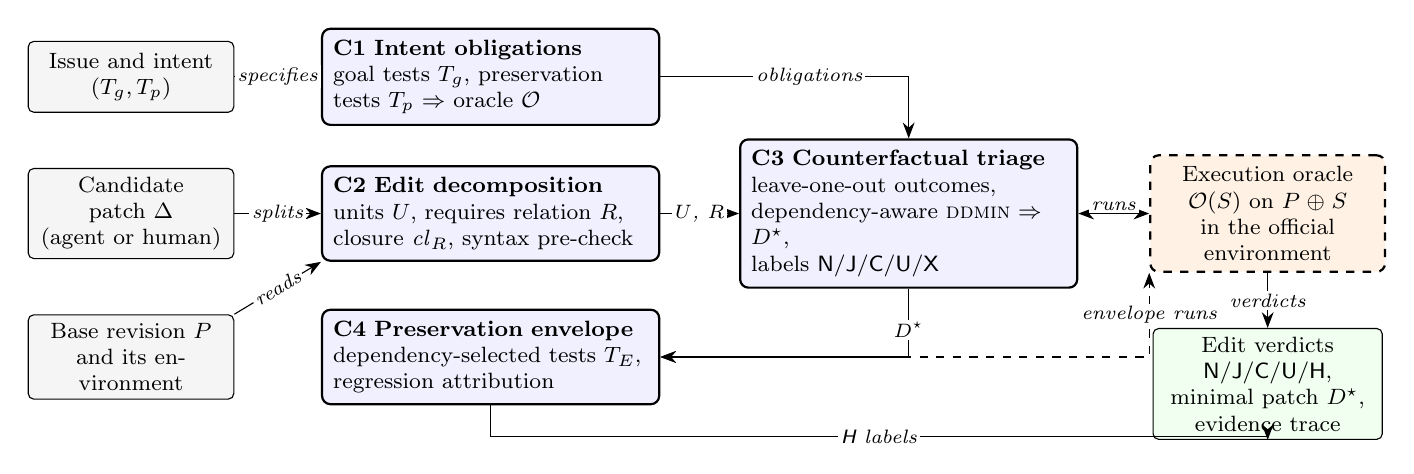
\begin{tikzpicture}[
  font=\footnotesize, >={Stealth[length=2mm]},
  io/.style={draw, rounded corners=2pt, fill=black!4, align=center, minimum height=9mm, inner sep=3pt, text width=24mm},
  comp/.style={draw, thick, rounded corners=3pt, fill=blue!6, align=left, inner sep=4pt, text width=40mm},
  orc/.style={draw, dashed, thick, rounded corners=3pt, fill=orange!10, align=center, inner sep=4pt, text width=27mm},
  el/.style={fill=white, inner sep=1pt, font=\scriptsize\itshape}]
\node[io] (issue) {Issue and intent\\$(T_g, T_p)$};
\node[io, below=7mm of issue] (patch) {Candidate patch $\Delta$\\(agent or human)};
\node[io, below=7mm of patch] (base) {Base revision $P$\\and its environment};
\node[comp, right=11mm of issue] (c1) {\textbf{C1 Intent obligations}\\goal tests $T_g$, preservation\\tests $T_p$ $\Rightarrow$ oracle $\mathcal{O}$};
\node[comp, right=11mm of patch] (c2) {\textbf{C2 Edit decomposition}\\units $U$, requires relation $R$,\\closure $\mathit{cl}_R$, syntax pre-check};
\node[comp, right=11mm of base] (c4) {\textbf{C4 Preservation envelope}\\dependency-selected tests $T_E$,\\regression attribution};
\node[comp, right=10mm of c2] (c3) {\textbf{C3 Counterfactual triage}\\leave-one-out outcomes,\\dependency-aware \textsc{ddmin} $\Rightarrow D^\star$,\\labels \lab{N}/\lab{J}/\lab{C}/\lab{U}/\lab{X}};
\node[orc, right=9mm of c3] (orc) {Execution oracle\\$\mathcal{O}(S)$ on $P\oplus S$\\in the official\\environment};
\node[io, below=7mm of orc, text width=27mm, fill=green!6] (out) {Edit verdicts\\\lab{N}/\lab{J}/\lab{C}/\lab{U}/\lab{H},\\minimal patch $D^\star$,\\evidence trace};
\draw[->] (issue) -- node[el]{specifies} (c1);
\draw[->] (patch) -- node[el]{splits} (c2);
\draw[->] (base.north east) -- node[el, sloped]{reads} (c2.south west);
\draw[->] (c1.east) -| node[el, pos=.3]{obligations} (c3.north);
\draw[->] (c2) -- node[el]{$U$, $R$} (c3);
\draw[<->] (c3) -- node[el, above]{runs} (orc);
\draw[->] (c3.south) |- node[el, pos=.3]{$D^\star$} (c4.east);
\draw[<->, dashed] (c4.east) -| node[el, pos=.75]{envelope runs} (orc.south west);
\draw[->] (c4.south) -- ++(0,-4mm) -| node[el, pos=.25]{\lab{H} labels} (out.south);
\draw[->] (orc) -- node[el]{verdicts} (out);
\end{tikzpicture}}
\caption{Overview of \tool{}. C1 turns the intent into test obligations. C2 splits the patch into units and computes which units require others. C3 withdraws units counterfactually and searches for a minimal sufficient subset $D^\star$, labelling every unit necessary (\lab{N}), jointly needed (\lab{J}), coupled (\lab{C}), unneeded (\lab{U}) or unresolved (\lab{X}). C4 runs additional dependency-selected tests to expose behaviour changes outside $T_p$ and attributes them to units (\lab{H}, harmful). The execution oracle (dashed) is independent of \tool{}: it is the instance's official environment and test command.}
\label{fig:overview}
\end{figure*}

A single invocation proceeds as follows. C1 fixes the obligations: the goal tests $T_g$ and the preservation tests $T_p$ (Section~\ref{sec:intent}). C2 splits $\Delta$ into units and computes a \emph{requires} relation that records, for example, that a unit calling a new helper needs the unit that defines it (Section~\ref{sec:decomp}). C3 first checks that the full patch is valid and that the base revision is not. It then withdraws each unit in turn and runs a dependency-aware \textsc{ddmin} to find a closed 1-minimal sufficient subset $D^\star$. Each unit receives a label from these two experiments (Section~\ref{sec:triage}). C4 selects test modules that exercise the edited modules but are not part of $T_p$, runs them on the base revision, on the reference behaviour and on the patched program, and attributes any new failure to the responsible units (Section~\ref{sec:envelope}). Optionally, the per-unit verdicts can be compared with claims that a reviewer, human or LLM, makes about the same edits. We use this comparison in the evaluation (RQ2).

\tool{} reuses three established ideas: atomic changes from CIA~\citep{ren2004chianti}, \textsc{ddmin}~\citep{zeller2002ddmin} and static regression test selection~\citep{rothermel1997safe}. Its contribution is the combination into an outcome-relative edit triage with explicit labels and guarantees, and the empirical demonstration that this judgment differs from location-based judgments on agent patches.

\subsection{C1: Intent obligations}\label{sec:intent}
\emph{Why needed.} Location-based review has no explicit statement of what the change must achieve, so it falls back on where the change is. \tool{} makes the outcome explicit. \emph{Contract.} Input: an intent specification. Output: the oracle $\mathcal{O}$ of Definition~\ref{def:oracle} and the environment in which it runs.

An intent specification names the goal behaviour, the behaviour to preserve, and how both are checked. Listing~\ref{lst:spec} shows the specification of the running example in a small declarative notation. The \code{objective} block lists the goal tests. The \code{preserve} block lists the preservation tests and asks for an envelope (C4) around the edited modules. The \code{evidence} block states which experiments \tool{} must run. Only the executable parts (test identifiers and envelope parameters) are compiled into $\mathcal{O}$. Free-text descriptions are kept for the reviewer and are never treated as evidence.

\begin{lstlisting}[float=t,basicstyle=\ttfamily\scriptsize,frame=single,numbers=none,caption={Intent specification for the running example. Only test identifiers and envelope parameters are compiled into the oracle; the note is for human readers.},label=lst:spec]
intent django__django-13297 {
  objective {                                   // goal tests T_g
    test generic_views.test_base.DeprecationTests.test_template_params_filtering
  }
  preserve {                                    // preservation tests T_p
    tests  instance.PASS_TO_PASS                 // 52 tests in generic_views.test_base
    envelope import_rts(k = 6)                  // C4: dependency-selected tests
  }
  evidence {
    rerun full_patch times 2                    // flakiness check
    counterfactual leave_one_out, minimise      // C3
  }
  note "URL kwargs wrapped for deprecation must remain usable as query parameters"
}
\end{lstlisting}


\emph{Properties.} The oracle is deterministic only up to test flakiness~\citep{luo2014flaky}. \tool{} therefore re-executes the full patch and treats an inconsistent outcome as \lab{X} for the whole patch rather than guessing.

\subsection{C2: Edit decomposition and the requires relation}\label{sec:decomp}
\emph{Why needed.} Withdrawing an arbitrary subset of units can produce a program that does not even load, for example when a call to a new helper is kept but the helper's definition is withdrawn. Such configurations waste oracle executions and, worse, can make a unit look necessary merely because its removal breaks name binding. \emph{Contract.} Input: $\Delta$ and $P$. Output: units $U$, a requires relation $R\subseteq U\times U$ and a cheap syntactic pre-check.

\begin{definition}[Requires relation and closure]\label{def:requires}
For units $a\neq b$, $(a,b)\in R$ (``$a$ requires $b$'') if (i) the lines added by $a$ use a name that $b$ newly binds, that is, a name not bound in the base version of $b$'s file, or (ii) $a$ removes the binding of a name whose remaining uses are removed by $b$. Because Python binds imports and assignments per module, bindings of these kinds relate only units of the same file, whereas new functions and classes may relate units of different files. The closure $\mathit{cl}_R(S)$ is the smallest superset of $S$ that contains $b$ whenever it contains $a$ and $(a,b)\in R$.
\end{definition}

$R$ over-approximates binding dependencies by name matching. It may add a unit that is not strictly required, which only makes the evaluated configuration larger, but it never removes a unit. All oracle calls of C3 are made on closed configurations $\mathit{cl}_R(S)$. Before each call, the pre-check parses every resulting Python file. A configuration that does not parse is labelled \lab{invalid} without running tests.

\emph{Running example.} The patch of Figure~\ref{fig:example} has four units. Unit u2 uses \code{LazyObject}, which u1 imports into \code{operations.py}, and u4 uses the name that u3 adds to the import in \code{fields/__init__.py}. Hence $R=\{(u_2,u_1),(u_4,u_3)\}$. Both files import the same name, but Python binds imports per module, so an earlier version of our relation that matched names across files linked $u_2$ to $u_3$ and $u_4$ to $u_1$ and made the unneeded import $u_1$ look necessary. Scoping import and assignment bindings to their file removes this artefact. Every subset of the four units parses, so the pre-check rejects nothing here.


\subsection{C3: Counterfactual triage}\label{sec:triage}
\emph{Why needed.} A passing test run tells us that the patch as a whole meets the obligations. It does not tell us which units contribute. \emph{Contract.} Input: $U$, $R$ and $\mathcal{O}$. Output: a label per unit and a sufficient subset $D^\star\subseteq U$.

\tool{} performs two complementary counterfactual experiments. The \emph{leave-one-out} experiment withdraws one unit together with the units that require it and observes the outcome. It identifies units that are individually indispensable. It cannot detect redundancy: if two units each repair the defect on their own, neither is individually indispensable, yet one of them is needed. The \emph{minimisation} experiment runs \textsc{ddmin} over the units, with the polarity reversed so that ``interesting'' means \emph{valid}, and with every configuration closed under $R$. Its result $D^\star$ is a sufficient subset in which every unit is needed given the others.

\begin{definition}[Edit labels]\label{def:labels}
Let $\mathit{Valid}(U)$ hold and $\mathit{Valid}(\emptyset)$ not hold. Let $\mathit{dep}(u)$ be the units that transitively require $u$, $o_u=\mathcal{O}(U\setminus(\{u\}\cup\mathit{dep}(u)))$ the leave-one-out outcome of $u$, and $D^\star$ the sufficient subset returned by Algorithm~\ref{alg:triage}. A unit $u$ is
\begin{itemize}
\item \lab{X} (\emph{unresolved}) if $o_u=\lab{error}$, and otherwise
\item \lab{N} (\emph{necessary}) if $o_u\neq\lab{valid}$ and $u\in D^\star$;
\item \lab{J} (\emph{jointly needed}) if $o_u=\lab{valid}$ and $u\in D^\star$;
\item \lab{C} (\emph{coupled}) if $o_u\neq\lab{valid}$ and $u\notin D^\star$;
\item \lab{U} (\emph{unneeded}) if $o_u=\lab{valid}$ and $u\notin D^\star$.
\end{itemize}
A unit is \emph{needed} if it is \lab{N} or \lab{J}, and \emph{removable} if it is \lab{U} or \lab{C}.
\end{definition}

The \lab{C} label captures a case that leave-one-out alone misreads. Two units can depend on each other behaviourally without a name-binding relation, for instance when one removes a decorator and the other compensates for that removal elsewhere. Withdrawing either one alone breaks the obligations, so both look indispensable, yet withdrawing both restores validity. Such units are removable as a group, and \tool{} reports them as coupled rather than necessary.

\begin{algorithm}[t]
\caption{Counterfactual triage (C3)}\label{alg:triage}
\begin{algorithmic}[1]
\Require units $U$, requires relation $R$, oracle $\mathcal{O}$ (memoised, closed under $R$, with syntax pre-check)
\Ensure labels $L: U\to\{\lab{N},\lab{J},\lab{C},\lab{U},\lab{X}\}$ and sufficient subset $D^\star$
\If{$\neg\mathit{Valid}(U)$ \textbf{or} \Call{Rerun}{$U$} $\neq\lab{valid}$ \textbf{or} $\mathit{Valid}(\emptyset)$} \State \Return \Call{Unresolved}{$U$} \EndIf
\For{each $u\in U$}
  \State $o_u \gets \mathcal{O}(U\setminus(\{u\}\cup\mathit{dep}(u)))$ \Comment{leave-one-out}
\EndFor
\State $D \gets \mathit{cl}_R(\Call{DDMin}{U, \mathit{Valid}\circ\mathit{cl}_R})$ \Comment{reversed polarity}
\While{some $u\in D$ has $\mathit{Valid}(\mathit{cl}_R(D\setminus(\{u\}\cup\mathit{dep}(u))))$}
  \State $D \gets \mathit{cl}_R(D\setminus(\{u\}\cup\mathit{dep}(u)))$ \Comment{closure-aware reduction}
\EndWhile
\State $D^\star\gets D$
\For{each $u\in U$} \State $L(u)\gets$ \Call{Label}{$o_u$, $u\in D^\star$} \Comment{Definition~\ref{def:labels}} \EndFor
\State \Return $L, D^\star$
\end{algorithmic}
\end{algorithm}

\textsc{DDMin} is the algorithm of \citet{zeller2002ddmin}. It repeatedly partitions the current configuration, tries each part and each complement, keeps the first one that is still valid, and refines the partition when none is. Because \textsc{DDMin} tests closures, a unit can enter its result only because another unit requires it, and the result can then contain a unit whose withdrawal is harmless. The reduction loop removes such units: they withdraw one unit together with the units that require it, and keep the smaller configuration whenever it remains valid. Every call goes through the memoised oracle, so configurations already evaluated are not executed again.

\begin{proposition}[Closed 1-minimality]\label{prop:min}
Under a deterministic oracle, $D^\star$ is valid, and for every $u\in D^\star$ the configuration $\mathit{cl}_R(D^\star\setminus(\{u\}\cup\mathit{dep}(u)))$ is not valid.
\end{proposition}
\begin{proof}
$D^\star$ is valid because \textsc{DDMin} accepts only configurations whose closure the oracle judged valid, and the reduction loop replaces $D$ only by a configuration it has just judged valid. The loop terminates because $D$ strictly shrinks in each iteration (the withdrawn unit $u$ is not added back by closure, since every unit that requires $u$ is withdrawn with it and $\mathit{cl}_R$ adds only units required by the remaining ones). On termination, its guard is false for every $u\in D^\star$, which is the claim.
\end{proof}

\begin{proposition}[Soundness of labels relative to the oracle]\label{prop:sound}
Assume $\mathcal{O}$ is deterministic. (a) If $L(u)=\lab{N}$, the largest closed configuration that omits $u$, namely $U\setminus(\{u\}\cup\mathit{dep}(u))$, is not valid. (b) If $L(u)\in\{\lab{U},\lab{C}\}$, there exists a valid configuration, $D^\star$, that does not contain $u$.
\end{proposition}
\begin{proof}
(a) A closed configuration that omits $u$ must omit every unit of $\mathit{dep}(u)$, since each of them requires $u$ transitively and closure would otherwise add $u$. The largest such configuration is $U\setminus(\{u\}\cup\mathit{dep}(u))$, and the oracle judged it not valid ($o_u\neq\lab{valid}$). (b) By Proposition~\ref{prop:min}, $D^\star$ is valid, and $u\notin D^\star$ by the definition of the labels.
\end{proof}


The guarantees are relative to the oracle. A label \lab{U} means that the obligations are met without the unit. It does not mean that the unit is useless to a human reader, nor that it is behaviour-neutral outside $T_g\cup T_p$. The envelope (C4) addresses the second point. Labels can also depend on the order in which \textsc{ddmin} explores subsets when several minimal subsets exist. \tool{} reports such units as \lab{J} or \lab{U} consistently with the $D^\star$ it found, and RQ4 compares $D^\star$ with exhaustive search on small patches.

\emph{Cost.} The leave-one-out loop needs $|U|$ oracle calls. \textsc{ddmin} needs $O(|U|^2)$ calls in the worst case and $O(\log |U|)$ when a single unit suffices~\citep{zeller2002ddmin}. Memoisation, closure and the syntax pre-check reduce the number of test executions further (RQ4).

\emph{Running example.} The full patch passes the goal test and all 52 preservation tests twice, and the base revision fails the goal test. Leave-one-out withdraws each unit with its dependents: withdrawing $u_1$ (and therefore $u_2$) or $u_2$ alone leaves the patch valid, while withdrawing $u_3$ (with $u_4$) or $u_4$ makes the goal test fail. \textsc{DDMin} then finds $D^\star=\{u_3,u_4\}$, which is valid, and the reduction loop cannot shrink it further. The labels are therefore $u_1{:}\,\lab{U}$, $u_2{:}\,\lab{U}$, $u_3{:}\,\lab{N}$, $u_4{:}\,\lab{N}$, obtained with \exOracleCalls{} oracle executions. The fix the agent relies on is the two-line unwrapping in \code{Field.get_prep_value}. The change to the database backend's value adapter, which the agent described in a comment as the place that forces evaluation, is not needed for any obligation. This judgement does not depend on the location of the edits: all four lie outside the reference patch, two are needed and two are not. Necessity is also distinct from correctness. Unit $u_4$ reads the private attribute \code{_wrapped}, and whether that is acceptable is a question for the reviewer that no test obligation answers.


\subsection{C4: Preservation envelope and attribution}\label{sec:envelope}
\emph{Why needed.} The preservation tests $T_p$ of a benchmark instance are usually drawn from the test files that the reference fix touched. An edit outside those files can change behaviour that no test in $T_p$ observes, and C3 would label it \lab{U} although it is harmful. \emph{Contract.} Input: the edited modules, $D^\star$ and the repository's test suite. Output: regressions outside $T_p$ and the units responsible.

C4 performs a static, import-based regression test selection. A test module receives a score for importing an edited module (3), for a matching file name (3), for residing in the same directory as an instance test file (2), for sharing a non-generic package name with an edited module (2) and for importing the parent package of an edited module (1). The top $k$ modules with score at least 2 form the envelope $T_E$ ($k=6$ in our evaluation). The selection is deliberately cheap and approximate. Its ability to expose changes is measured, not assumed (RQ3).

\begin{algorithm}[t]
\caption{Preservation envelope and attribution (C4)}\label{alg:envelope}
\begin{algorithmic}[1]
\Require base $P$, reference behaviour $P_{\mathit{ref}}$, units $U$, sufficient subset $D^\star$, envelope tests $T_E$
\Ensure regressions $\mathit{Reg}$ and harmful units $H$
\State $\mathit{Stable} \gets \Call{Pass}{P, T_E} \cap \Call{Pass}{P, T_E}$ \Comment{two runs; flaky tests excluded}
\State $\mathit{Intended} \gets \mathit{Stable}\setminus\Call{Pass}{P_{\mathit{ref}}, T_E}$ \Comment{behaviour the reference also changes}
\State $\mathit{Reg} \gets \mathit{Stable}\setminus\Call{Pass}{P\oplus U, T_E}\setminus\mathit{Intended}\setminus T_g$
\If{$\mathit{Reg}=\emptyset$} \Return $\emptyset, \emptyset$ \EndIf
\State $\mathit{Reg}_{D} \gets \mathit{Reg}\setminus\Call{Pass}{P\oplus D^\star, T_E}$ \Comment{caused by needed units}
\State $H \gets \emptyset$
\For{each $u\in U\setminus D^\star$}
  \If{$(\mathit{Reg}\setminus\mathit{Reg}_D)\setminus\Call{Pass}{P\oplus\mathit{cl}_R(D^\star\cup\{u\}), T_E}\neq\emptyset$} $H\gets H\cup\{u\}$ \EndIf
\EndFor
\State \Return $\mathit{Reg}, H$
\end{algorithmic}
\end{algorithm}

Algorithm~\ref{alg:envelope} compares outcomes on four programs: the base revision (twice, to discard flaky tests), the reference behaviour, the full patch and, if regressions appear, the sufficient subset $D^\star$ with each unneeded unit added back. A test whose outcome the reference fix also changes encodes intended behaviour and is excluded. Unneeded units that reintroduce a regression are labelled \lab{H} (\emph{harmful}). Regressions that persist in $D^\star$ alone are attributed to needed units, which signals a conflict between the goal and preservation rather than a removable edit. In deployment, $P_{\mathit{ref}}$ is unavailable. The step that removes intended changes is then replaced by human confirmation of the reported tests, and the remaining steps are unchanged.

\emph{Running example.} For the two edited database modules, C4 selects six test modules, among them \code{backends.base.test_operations} and the backend-specific operation tests, with 75 stable passing tests on the base revision. None of them changes outcome under the full patch, so no unit is labelled \lab{H}. The envelope therefore adds evidence that the unneeded units $u_1$ and $u_2$ do not change the tested behaviour of the database layer, which a reviewer may use to decide whether to keep them.

\emph{Claims versus evidence in the running example.} We asked five open-weight LLMs to judge the four units (Section~\ref{sec:setup}). All five call $u_2$ a \emph{fix} and $u_1$ a \emph{support} edit, and all of them judge $u_2$ needed in every sample. The agent's own comment on $u_2$ (``Force evaluation of the lazy object'') makes this explanation plausible. Counterfactual execution shows that it is not what the tests rely on.


\subsection{Comparing claims with evidence}\label{sec:claims}
Reviewers, and increasingly LLMs, explain patches by stating which edit fixes the defect, which supports the fix and which is incidental. \tool{} treats such statements as \emph{claims}. Given the same units that \tool{} analyses, a reviewer can propose repair hypotheses and assign each unit a hypothesis, a role and a needed/not-needed judgment. The counterfactual labels provide a reference against which these claims are checked. We use this comparison in RQ2 to ask whether LLM reviewers can stand in for counterfactual evidence. The comparison is one-directional: claims never change \tool{}'s labels.

\section{Evaluation}\label{sec:evaluation}

\subsection{Experimental setup}\label{sec:setup}

\paragraph{Research questions.} The evaluation tests the claims of the introduction through four research questions.
\begin{description}
\item[RQ1 (Footprint)] How do the exploration and edit footprints of LLM agents differ from the human reference patches for the same issues, and how are footprint properties associated with resolution?
\item[RQ2 (Necessity)] What fraction of the edits in resolved agent patches is counterfactually needed, and how well do location-, dependency- and LLM-judgement-based proxies recover edit necessity?
\item[RQ3 (Preservation)] Does the preservation envelope expose behaviour changes that the benchmark's regression tests miss, and does \tool{} attribute them to the responsible edits?
\item[RQ4 (Cost)] What does counterfactual triage cost, and how much do memoisation, the requires closure and the syntax pre-check reduce oracle executions relative to alternative strategies?
\end{description}
RQ1 is a descriptive study whose directional hypotheses (agents and humans differ in edit footprint) were fixed in advance. RQ2 and RQ3 are the primary tests of \tool{}. RQ4 characterises its cost. The protocol, including decision rules, was written before any \tool{} measurement and is part of the replication package. The protocol records seven dated amendments: four made before the affected measurements (LLM models available on the clusters, one unavailable cluster, architecture-related exclusions, one LLM excluded after its smoke test) and three corrections of the implementation found by consistency checks during execution, after which every affected record was re-run (Section~\ref{sec:threats}).

\paragraph{Benchmark and agent patches.} We use SWE-bench Verified~\citep{chowdhury2024verified} (500 instances from 12 Python repositories). Agent patches come from the public bash-only track of the SWE-bench leaderboard, in which every submission uses the same scaffold, mini-swe-agent~\citep{miniswe2025}, with a different LLM. Holding the scaffold fixed removes one major source of variation between systems. We downloaded the submitted patch, the official evaluation report and, where published, the full trajectory of every system. RQ1 includes every system with at least 450 patch files (\rqoneSystems{} systems). For RQ2--RQ4 we fixed in advance an execution panel of eight systems spanning vendors, open and closed weights, and capability (Table~\ref{tab:panel}).

% BEGIN:panel-table
\begin{table}[t]
\caption{Execution panel. \emph{Resolved (Verified)}: official resolution rate on all 500 instances. \emph{Candidates}: officially resolved patches on the 295 validated Django and SymPy instances. \emph{Valid}: patches that also resolve in our environment and were triaged. \emph{Not valid}: patches that did not reproduce their resolution. \emph{Other}: flaky or erroneous runs. $^\dagger$Open weights.}
\label{tab:panel}
\centering\footnotesize
\begin{tabular}{lrrrrrr}
\toprule
System & Resolved (Verified) & Candidates & Valid & Not valid & Other & Units \\
\midrule
Claude 4.6 Opus & 76.8\% & 229 & 198 & 0 & 0 & 442 \\
GPT-5.2 (high) & 72.8\% & 223 & 193 & 0 & 0 & 630 \\
Gemini 3 Pro (high) & 74.0\% & 207 & 191 & 0 & 0 & 427 \\
Kimi K2.5 (high)$^\dagger$ & 71.5\% & 222 & 194 & 0 & 0 & 391 \\
DeepSeek V3.2 (high)$^\dagger$ & 70.1\% & 219 & 191 & 0 & 0 & 469 \\
GPT-5 mini & 58.8\% & 174 & 154 & 0 & 0 & 274 \\
Qwen2.5-Coder 32B$^\dagger$ & 9.8\% & 28 & 22 & 0 & 0 & 49 \\
GPT-4o & 23.6\% & 79 & 66 & 2 & 0 & 256 \\
Reference (human) & -- & 295 & 252 & 0 & 0 & 793 \\
\bottomrule
\end{tabular}
\end{table}
% END:panel-table

\paragraph{Execution subset and oracle.} Counterfactual triage requires executing tests many times per patch. We restricted RQ2--RQ4 to the Django and SymPy instances (306 of 500), which together make up 61\% of SWE-bench Verified. We rebuilt their official SWE-bench 4.0.4 environments natively for \texttt{linux/arm64}. Ten instances are pinned to \texttt{x86\_64} by the harness and were excluded. We then validated every remaining environment with the reference patch: 295 of 296 resolve (one Django reference patch fails on arm64 and was excluded). For each validated instance, the panel's officially resolved patches and the reference patch form the analysed set. A patch that does not reproduce its resolution in our environment is reported as \lab{not valid} and excluded from the label statistics.

\paragraph{Proxies and LLM judges (RQ2).} We compare \tool{}'s labels with four location-based proxies that predict whether a source edit is needed: \emph{gold-file} (the edit is in a file that the reference patch modifies), \emph{issue-mention} (the issue text names the file, its module path or its base name), \emph{import-proximity} (the edited module is at most one import hop from a reference-patch module) and \emph{all-needed} (every edit is needed, the implicit assumption of whole-patch acceptance). We also use five open-weight LLMs as reviewers: Qwen2.5-Coder 7B, Llama~3.1 8B, Gemma~2 9B, Phi-4 14B and Mistral Small 24B. Each receives the issue and the patch split into the same units that \tool{} analyses, and returns repair hypotheses and, for each unit, a hypothesis, a role and a needed/not-needed judgement in a JSON schema. We sample three generations per patch (temperature 0.2, seeds 11, 22 and 33) and take the majority vote.

\paragraph{Injection study (RQ3).} Real regressions outside the benchmark tests are rare and have no ground truth, so we complement them with a controlled study. For every validated instance we append one unit to the reference patch in a module that the reference does not edit but that lies within two import hops of an edited module. The unit is either \emph{semantic} (relational-operator flip, condition negation, integer-constant increment, or return-value replacement by \code{None}) or \emph{neutral} (an added comment, redundant parentheses around a return value, or an unused local assignment). Mutation operators of this kind are standard proxies for real faults~\citep{jia2011mutation,just2014mutants}. Operator, module and site are drawn from a seeded generator. The expected outcome is known by construction: a neutral unit must be labelled \lab{U} and never \lab{H}, and a semantic unit should be detected by the official tests or by the envelope.

\paragraph{Metrics.} RQ1 measures, per patch, the number of edited source files, change blocks (units in source files), source churn (added plus removed lines), the number of auxiliary files (files outside the package and its tests, such as reproduction scripts), the share of source change blocks in files that the reference patch does not edit (\emph{nonlocal share}), and \emph{dispersion}, the mean pairwise distance between edited source modules in the undirected module-import graph of the base revision. From trajectories we count the distinct repository files referenced by the agent's commands and the \emph{exploration-to-edit ratio} (referenced files per edited file). RQ2 reports label shares, precision, recall and F1 for flagging unneeded edits, the Matthews correlation coefficient (MCC)~\citep{chicco2020mcc} for the needed/unneeded decision, and the \emph{nonlocal-needed retention} of each proxy: the fraction of needed edits outside reference-patch files that the proxy classifies as needed. RQ3 reports the fraction of patches with envelope regressions and, for the injection study, detection rates by official tests and by official tests plus envelope. RQ4 counts oracle executions, syntax pre-check rejections and wall-clock time.

\paragraph{Statistical analysis.} The experimental unit is a patch (system $\times$ instance), and edits are nested in patches, which are nested in instances. All confidence intervals are 95\% percentile intervals from a bootstrap that resamples instances (10{,}000 resamples for proportions, 2{,}000 for classification metrics). For RQ1, we compare each system with the reference patch on the same instances using the Wilcoxon signed-rank test, report as effect size the matched-pairs rank-biserial correlation $r=(W^{+}-W^{-})/(W^{+}+W^{-})$, where $W^{+}$ and $W^{-}$ are the rank sums of positive and negative differences ($r\in[-1,1]$, positive when the agent value is larger), and apply the Holm correction across systems within each metric~\citep{holm1979}. The pre-registered decision rule supports a directional difference for a metric if at least two thirds of the systems show a Holm-significant difference in the same direction. The association between footprint and resolution is estimated with a logistic generalised estimating equation (GEE) clustered by instance~\citep{liang1986gee}, and is exploratory.

\subsection{Implementation}\label{sec:impl}
\tool{} is implemented in Python (about 1{,}500 lines for the approach and 1{,}000 for experiments and analysis) with 80 unit and property-based tests. Patch parsing uses \code{unidiff}. Hunks are located by exact match of their pre-image nearest to the declared line, which reproduces the offset tolerance of \code{git apply}. The oracle reuses the SWE-bench 4.0.4 environment specifications, test commands and log parsers without modification. For each analysed patch, \tool{} starts one container from the instance image, applies and commits the instance's test patch once, and then, for every configuration, hard-resets the working tree, writes the configured file contents and runs the instance's test command. Containers run without network access, with two CPUs and 8\,GB of memory, and a 900-second timeout per test run. Instance images were built locally for \texttt{linux/arm64} from the official specifications. Repository clones were served to the image builds from local mirrors, and every build still resets to the instance's pinned base commit.

All execution ran on one workstation (NVIDIA GB10, 20 Arm cores, 121\,GB memory) with up to 15 patches analysed in parallel. The LLM judges ran on two Digital Research Alliance of Canada clusters, Rorqual (NVIDIA H100 80\,GB) and Narval (NVIDIA A100), with one GPU per model and a node-local Ollama 0.32.14 server. Before any prompt was sent, each job loaded the model, verified full GPU residency and recorded the model digest. Every request and response, with timing and token counts, is stored. We smoke-tested every model on both clusters with 24 prompts before the full runs and submitted each full run with a Slurm dependency on the success of its smoke test. The study used \nGpuJobs{} Slurm jobs and \nGpuHours{} GPU-hours (\nGpuHoursRorqual{} on Rorqual, \nGpuHoursNarval{} on Narval) to produce \nLlmGenerations{} judge responses. One planned model, DeepSeek-Coder-V2 16B, was excluded after its smoke test because the runtime processed prompts at CPU speed on the H100 and returned no parseable answer. A third cluster (Fir) was unavailable during the study window because its login node denied access to the file systems.

\subsection{RQ1: Edit and exploration footprints}\label{sec:rq1}
\emph{Design.} For each of the \rqoneSystems{} systems we compare its patch with the reference patch on the same instances (\rqonePatches{} agent patches in total). Figure~\ref{fig:rq1} relates each system's resolution rate to where it edits, and Table~\ref{tab:explore} summarises exploration for the panel.

% BEGIN:rq1-figure
\begin{figure}[pos=htbp]
\centering
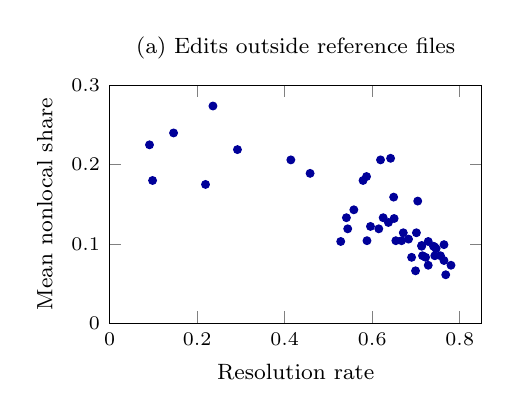
\begin{tikzpicture}
\begin{axis}[width=0.52\linewidth, height=4.6cm, xlabel={Resolution rate}, ylabel={Mean nonlocal share},
  xmin=0, xmax=0.85, ymin=0, ymax=0.3, tick label style={font=\scriptsize}, label style={font=\footnotesize},
  title={(a) Edits outside reference files}, title style={font=\footnotesize}]
\addplot[only marks, mark=*, mark size=1.4pt, blue!60!black] coordinates {(0.219,0.175) (0.091,0.225) (0.236,0.274) (0.649,0.159) (0.146,0.240) (0.544,0.119) (0.596,0.122) (0.458,0.189) (0.704,0.154) (0.579,0.180) (0.098,0.180) (0.654,0.104) (0.615,0.119) (0.414,0.206) (0.292,0.219) (0.541,0.133) (0.558,0.143) (0.713,0.097) (0.743,0.085) (0.667,0.104) (0.756,0.085) (0.699,0.066) (0.642,0.208) (0.683,0.106) (0.619,0.206) (0.587,0.185) (0.637,0.127) (0.625,0.133) (0.650,0.132) (0.690,0.083) (0.722,0.083) (0.528,0.103) (0.671,0.114) (0.780,0.073) (0.713,0.098) (0.768,0.061) (0.701,0.114) (0.764,0.099) (0.740,0.097) (0.746,0.094) (0.728,0.103) (0.588,0.104) (0.715,0.085) (0.764,0.079) (0.728,0.073) (0.743,0.096)};
\end{axis}
\end{tikzpicture}\hfill
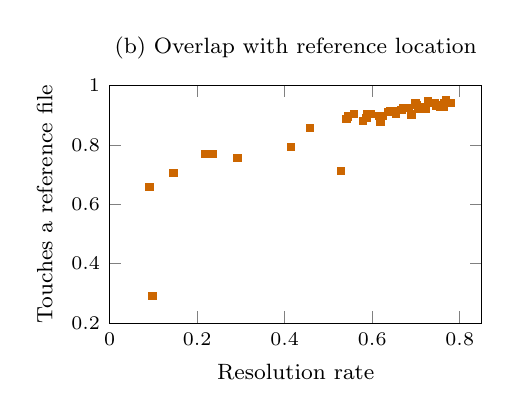
\begin{tikzpicture}
\begin{axis}[width=0.52\linewidth, height=4.6cm, xlabel={Resolution rate}, ylabel={Touches a reference file},
  xmin=0, xmax=0.85, ymin=0.2, ymax=1, tick label style={font=\scriptsize}, label style={font=\footnotesize},
  title={(b) Overlap with reference location}, title style={font=\footnotesize}]
\addplot[only marks, mark=square*, mark size=1.3pt, orange!80!black] coordinates {(0.219,0.770) (0.091,0.658) (0.236,0.770) (0.649,0.912) (0.146,0.705) (0.544,0.895) (0.596,0.904) (0.458,0.857) (0.704,0.921) (0.579,0.881) (0.098,0.291) (0.654,0.905) (0.615,0.897) (0.414,0.793) (0.292,0.755) (0.541,0.886) (0.558,0.903) (0.713,0.925) (0.743,0.940) (0.667,0.917) (0.756,0.929) (0.699,0.939) (0.642,0.914) (0.683,0.923) (0.619,0.878) (0.587,0.890) (0.637,0.910) (0.625,0.898) (0.650,0.910) (0.690,0.902) (0.722,0.920) (0.528,0.711) (0.671,0.924) (0.780,0.941) (0.713,0.928) (0.768,0.949) (0.701,0.934) (0.764,0.940) (0.740,0.940) (0.746,0.932) (0.728,0.948) (0.588,0.902) (0.715,0.927) (0.764,0.929) (0.728,0.944) (0.743,0.941)};
\end{axis}
\end{tikzpicture}
\caption{Location of agent edits relative to the reference patch for the 46 mini-swe-agent systems (one point per system, SWE-bench Verified). (a) Mean share of source change blocks in files the reference patch does not edit. (b) Share of patches that edit at least one reference-patch file. Spearman $\rho$ with the resolution rate: -0.83 in (a) and 0.94 in (b).}
\label{fig:rq1}
\end{figure}
% END:rq1-figure

\emph{Results.} Agent patches are \emph{not} broader than human patches. Against the pre-registered rule (two thirds of systems, i.e., at least 31 of \rqoneSystems{}), no size metric supports the hypothesis that agents edit more. Agents edit significantly fewer source files than the reference in \rqoneFilesLess{} systems and more in \rqoneFilesGreater{} (median $r=\rqoneFilesMedR$). They produce significantly fewer source change blocks in \rqoneBlocksLess{} systems and more in \rqoneBlocksGreater{} (median $r=\rqoneBlocksMedR$, reference mean \rqoneGoldBlocks{} blocks). Their edits are less dispersed over the import graph in \rqoneDispLess{} systems and more dispersed in none. Churn is mixed (\rqoneChurnGreater{} systems higher, \rqoneChurnLess{} lower). The only metric that meets the decision rule is the number of auxiliary files, such as reproduction scripts left in the repository root (\rqoneAuxGreater{} systems). This difference, however, is a property of the scaffold rather than of the models: none of the \rqoneVtwoSystems{} systems run with mini-swe-agent~2.0 leave auxiliary files (\rqoneVtwoAuxGreater{} significant), whereas earlier scaffold versions submit untracked files with the patch.

Where agents edit matters more than how much they edit. Across systems, the mean share of edits outside reference-patch files falls as the resolution rate rises (Spearman $\rho=\rqoneRhoNonlocal$, Figure~\ref{fig:rq1}a), and the share of patches that touch at least one reference file rises with it ($\rho=\rqoneRhoTouches$, Figure~\ref{fig:rq1}b). At the patch level, a logistic GEE clustered by instance confirms the association after controlling for system, churn and the number of edited files: each unit increase in nonlocal share multiplies the odds of resolution by \rqoneGeeNonlocalOR{} (95\% CI \rqoneGeeNonlocalLo--\rqoneGeeNonlocalHi), while churn ($p=\rqoneGeeChurnP$) and the number of files ($p=\rqoneGeeFilesP$) show no association.

% BEGIN:rq1-explore-table
\begin{table}[t]
\caption{Exploration footprint of the panel systems that publish trajectories (medians over SWE-bench Verified instances). \emph{Referenced}: distinct repository files named in the agent's shell commands (interquartile range in brackets). \emph{EER}: exploration-to-edit ratio, referenced files per edited file. GPT-4o's run has no published trajectories.}
\label{tab:explore}
\centering\footnotesize
\begin{tabular}{lrrrrrr}
\toprule
System & $n$ & Resolved & Steps & Referenced & Edited & EER \\
\midrule
Claude 4.6 Opus & 500 & 75.6\% & 25 & 3 [2--4] & 1 & 3.0 \\
GPT-5.2 (high) & 500 & 72.8\% & 33 & 3 [2--5] & 1 & 2.2 \\
Kimi K2.5 (high) & 500 & 70.8\% & 44 & 4 [3--6] & 1 & 4.0 \\
Gemini 3 Pro (high) & 495 & 70.3\% & 48 & 4 [3--6] & 1 & 4.0 \\
DeepSeek V3.2 (high) & 500 & 70.0\% & 83 & 6 [4--8] & 1 & 5.0 \\
GPT-5 mini & 500 & 56.2\% & 18 & 2 [1--3] & 1 & 2.0 \\
Qwen2.5-Coder 32B & 496 & 9.1\% & 32 & 1 [0--1] & 0 & 1.0 \\
\bottomrule
\end{tabular}
\end{table}
% END:rq1-explore-table

Exploration is broader than editing. The panel systems name a median of \rqoneExploreRefMin{} to \rqoneExploreRefMax{} repository files in their commands, but edit a median of one (Table~\ref{tab:explore}). Stronger systems do not explore less. DeepSeek V3.2 takes the most steps and references the most files at a resolution rate similar to the strongest systems.

\emph{Answer to RQ1.} Agent patches resemble human patches in size and are, if anything, more concentrated. Capable agents mostly edit where the human developer edited, and edits away from the reference location are associated with failure. Agents explore several files for every file they edit. These findings refine rather than confirm the starting hypothesis: the risk with agent patches is not sprawling edits but a minority of edits whose relevance a location-based reviewer cannot judge. RQ2 examines those edits.

\subsection{RQ2: Counterfactual necessity of agent edits}\label{sec:rq2}
\emph{Design.} We triaged every officially resolved panel patch and every reference patch on the validated instances (Table~\ref{tab:panel}). Of the \nCandidates{} candidate patches, \nValidPatches{} (\nAgentValid{} agent, \nGoldValid{} reference) reproduced their resolution and were labelled, \nNotValid{} did not reproduce it and \nOtherStatus{} ended as flaky or erroneous. We then compared the labels with the location proxies and the LLM judges. In this comparison, the counterfactual labels serve as the reference \emph{measurement} of necessity relative to the obligations, and the question is how well cheaper signals approximate it. RQ2 therefore does not evaluate \tool{} against itself: the validity of the labels rests on Propositions~\ref{prop:min} and~\ref{prop:sound} and on the injection study with known ground truth (RQ3). Because only resolved patches can be triaged, all necessity results describe successful patches.

% BEGIN:rq2-label-table
\begin{table}[t]
\caption{Counterfactual labels of the units of valid patches. \emph{Src U}: share of source units that are removable (\lab{U} or \lab{C}). \emph{Non-src}: units in test or auxiliary files. \emph{$\geq$1 removable}: share of patches with at least one removable unit.}
\label{tab:labels}
\centering\footnotesize
\begin{tabular}{lrrrrrrrrr}
\toprule
System & Patches & Units & \lab{N} & \lab{J} & \lab{C} & \lab{U} & Src U & Non-src & $\geq$1 removable \\
\midrule
Claude 4.6 Opus & 198 & 442 & 66.5\% & 0.2\% & 2.0\% & 31.2\% & 32.8\% & 3 & 19.7\% \\
GPT-5.2 (high) & 193 & 630 & 57.0\% & 0.2\% & 3.0\% & 39.8\% & 41.8\% & 11 & 35.2\% \\
Gemini 3 Pro (high) & 191 & 427 & 65.8\% & 0.0\% & 3.5\% & 30.7\% & 33.7\% & 3 & 22.0\% \\
Kimi K2.5 (high) & 194 & 391 & 77.7\% & 0.3\% & 1.3\% & 20.7\% & 21.4\% & 3 & 20.1\% \\
DeepSeek V3.2 (high) & 191 & 469 & 62.7\% & 0.0\% & 2.3\% & 35.0\% & 36.9\% & 3 & 34.6\% \\
GPT-5 mini & 154 & 274 & 78.8\% & 0.0\% & 0.0\% & 21.2\% & 21.2\% & 0 & 23.4\% \\
Qwen2.5-Coder 32B & 22 & 49 & 69.4\% & 0.0\% & 0.0\% & 30.6\% & 12.8\% & 10 & 31.8\% \\
GPT-4o & 66 & 256 & 28.9\% & 0.4\% & 0.4\% & 70.3\% & 35.3\% & 140 & 74.2\% \\
Reference (human) & 252 & 793 & 64.8\% & 0.0\% & 2.3\% & 32.9\% & 35.2\% & 0 & 24.6\% \\
\bottomrule
\end{tabular}
\end{table}
% END:rq2-label-table

\emph{How many edits are needed?} Most units of agent patches are needed, but a substantial minority are not (Table~\ref{tab:labels}). Across all valid agent patches, \rqtwoAgentShareN{} of units are necessary, \rqtwoAgentShareJ{} jointly needed, \rqtwoAgentShareC{} coupled and \rqtwoAgentShareU{} \rqtwoAgentShareUCI{} unneeded. \rqtwoAgentPatchesUnneeded{} \rqtwoAgentPatchesUnneededCI{} of agent patches contain at least one removable unit. Restricted to source code, \rqtwoAgentSrcUnneeded{} of agent units are removable. Units in test and auxiliary files are almost always removable (\rqtwoAgentTestUnneeded{} of \rqtwoAgentTestUnits{} test units and \rqtwoAgentAuxUnneeded{} of \rqtwoAgentAuxUnits{} auxiliary units), as expected: the instance's test patch overrides agent-written tests, and reproduction scripts are not on the tested path.

Reference patches are not a gold standard of necessity either. \rqtwoGoldShareU{} \rqtwoGoldShareUCI{} of their units and \rqtwoGoldSrcUnneeded{} of their source units are removable under their own F2P and P2P tests, and \rqtwoGoldPatchesUnneeded{} of reference patches contain at least one such unit. Typical cases are the same fix applied to a sibling code path that the tests do not exercise, or a defensive check added beside the fix. These edits may well be good engineering. The point is that a test-based oracle cannot see their value, and that treating the human patch as the definition of relevant code would count them as relevant by fiat.

\emph{Do location proxies recover necessity?} No. Table~\ref{tab:proxies} shows that the gold-file proxy flags almost none of the removable units (recall \rqtwoRecPgoldfile{}) and its MCC is \rqtwoMccPgoldfile{}. The reason is visible in the data: of the \rqtwoSrcUnneededN{} removable agent source units, \rqtwoUnneededInGold{} lie inside reference-patch files, exactly where a location-based reviewer would look for the fix. Import proximity behaves the same way (MCC \rqtwoMccPdep{}), and the issue-mention proxy flags more units but with low precision (MCC \rqtwoMccPissue{}). Conversely, \rqtwoNonlocalNeeded{} needed units lie outside reference-patch files, and the gold-file proxy misclassifies all of them as unneeded by construction. The high nonlocal retention of the LLM judges must be read together with their low recall: a judge that rarely calls any unit unneeded also rarely calls a nonlocal unit unneeded. Necessity and location are nearly independent: \rqtwoLocalNeededShare{} of agent source units inside reference files are needed, compared with \rqtwoNonlocalNeededShare{} outside them.

% BEGIN:rq2-proxy-table
\begin{table*}[t]
\caption{How well location proxies and LLM judges recover counterfactual necessity for the 2{,}765 source units of valid agent patches. Precision, recall and F1 refer to flagging \emph{removable} units. MCC refers to the needed/removable decision. Brackets: 95\% instance-cluster bootstrap intervals. \emph{Nonlocal retention}: share of the 50 needed units outside reference-patch files that the proxy classifies as needed. LLM judges: majority vote over three seeds.}
\label{tab:proxies}
\centering\footnotesize
\begin{tabular}{llrrrrr}
\toprule
Family & Proxy & Precision & Recall & F1 [95\% CI] & MCC [95\% CI] & Nonlocal retention \\
\midrule
Location & Gold-file & 0.83 & 0.26 & 0.40 [0.27, 0.52] & 0.36 [0.25, 0.46] & 0\% \\
Location & Issue-mention & 0.39 & 0.65 & 0.49 [0.38, 0.57] & 0.14 [0.03, 0.25] & 44\% \\
Location & Import-proximity & 0.89 & 0.19 & 0.31 [0.18, 0.45] & 0.33 [0.21, 0.43] & 56\% \\
Location & All-needed & -- & 0.00 & -- & -- & 100\% \\
\midrule
LLM judge & Gemma 2 9B & 0.77 & 0.16 & 0.27 [0.20, 0.34] & 0.25 [0.18, 0.34] & 100\% \\
LLM judge & Llama 3.1 8B & 0.31 & 0.30 & 0.31 [0.25, 0.37] & -0.01 [-0.09, 0.08] & 54\% \\
LLM judge & Mistral Small 24B & 0.91 & 0.27 & 0.41 [0.30, 0.53] & 0.40 [0.31, 0.50] & 100\% \\
LLM judge & Phi-4 14B & 0.92 & 0.18 & 0.31 [0.21, 0.42] & 0.34 [0.26, 0.43] & 100\% \\
LLM judge & Qwen2.5-Coder 7B & 0.49 & 0.36 & 0.41 [0.34, 0.49] & 0.19 [0.10, 0.31] & 86\% \\
\bottomrule
\end{tabular}
\end{table*}
% END:rq2-proxy-table

\emph{Can LLM judges stand in for counterfactual evidence?} Partly. The best judges (Phi-4 and Mistral Small) are precise when they call a unit unneeded (precision \rqtwoPrecLphib{} and \rqtwoPrecLmistralsmallb{}), but they call few units unneeded (recall \rqtwoRecLphib{} and \rqtwoRecLmistralsmallb{}), reaching MCC \rqtwoMccLphib{} and \rqtwoMccLmistralsmallb{}. The smaller Qwen2.5-Coder~7B flags more units at lower precision and attains the highest F1 (\rqtwoFoneLqwencoderb{}). Llama~3.1~8B is close to chance (MCC \rqtwoMccLllamab{}). All judges retain most nonlocal needed units, unlike the location proxies, because they reason about the issue rather than about file names. Their judgements are moderately stable across seeds (\rqtwoSeedAgreeMin--\rqtwoSeedAgreeMax{} of units receive the same judgement in all three samples) and almost always parseable (at least \rqtwoParseMin{} of responses).

\emph{Would the tests help the judges?} A judge that knows which tests define success might reason like the oracle. In an exploratory variant (one seed), we added the goal-test names and the instance's test patch to each prompt (Table~\ref{tab:informed}). The tests improve two judges (Phi-4 and Qwen2.5-Coder) and leave the others essentially unchanged, but recall stays at or below \rqtwoInfMaxRecall{} and the best MCC is \rqtwoInfMaxMcc{}. Reading the tests is not the same as executing them.

% BEGIN:rq2-informed-table
\begin{table}[pos=htbp]
\caption{Exploratory comparison (seed 11): LLM judges without and with the goal tests and the instance's test patch in the prompt. Precision and recall refer to flagging removable agent source units; MCC to the needed/removable decision.}
\label{tab:informed}
\centering\footnotesize
\begin{tabular}{lrrrrrr}
\toprule
 & \multicolumn{3}{c}{Issue and patch only} & \multicolumn{3}{c}{Plus goal tests} \\
\cmidrule(lr){2-4}\cmidrule(lr){5-7}
Judge & Prec. & Rec. & MCC & Prec. & Rec. & MCC \\
\midrule
Qwen2.5-Coder 7B & 0.48 & 0.34 & 0.18 & 0.59 & 0.46 & 0.33 \\
Llama 3.1 8B & 0.31 & 0.32 & 0.00 & 0.32 & 0.32 & -0.01 \\
Gemma 2 9B & 0.76 & 0.16 & 0.25 & 0.80 & 0.14 & 0.25 \\
Phi-4 14B & 0.90 & 0.18 & 0.33 & 0.96 & 0.25 & 0.41 \\
Mistral Small 24B & 0.91 & 0.32 & 0.45 & 0.95 & 0.27 & 0.43 \\
\bottomrule
\end{tabular}
\end{table}
% END:rq2-informed-table

\emph{Answer to RQ2.} About one in four source edits of resolved agent patches is not needed for the instance's obligations, and the same holds for a similar share of human reference edits. Location proxies cannot recover necessity because unneeded agent edits sit inside the files the reference patch edits. LLM judges are better and can serve as a cheap filter with high precision, but they miss most removable edits. Counterfactual execution remains necessary to establish what a patch needs.


\subsection{RQ3: Preservation envelope}\label{sec:rq3}
\emph{Design.} For every valid patch, C4 selected up to six test modules beyond the instance's own test files (median \rqthreeEnvTestsMedian{} stable passing tests per envelope). For \rqthreeEnvEmpty{} patches the selection found no qualifying module. We report regressions on the real patches and the outcomes of the injection study (\rqthreeSemanticN{} semantic and \rqthreeNeutralN{} neutral injections).

\emph{Real patches.} Envelope regressions are rare. They occur in \rqthreeAgentRegN{} agent patches (\rqthreeAgentRegRate{} \rqthreeAgentRegCI{}) and \rqthreeGoldRegN{} reference patches. In \rqthreeAgentHarmful{} agent patches \tool{} attributes a regression to a unit outside $D^\star$ (\lab{H}), so the regression disappears when that unit is removed. In \rqthreeAgentRegMinimal{} patches the regression persists in $D^\star$, which indicates a conflict between the obligations and preserved behaviour rather than a removable edit.

% BEGIN:rq3-injection-table
% END:rq3-injection-table

\emph{Injection study.} Table~\ref{tab:injection} shows that the official tests detect \rqthreeSemanticOfficial{} of semantic injections. Adding the envelope raises detection to \rqthreeSemanticEnvelope{}, an absolute gain of \rqthreeSemanticGain{}. Every detected injection is attributed to the injected unit. Neutral injections are never labelled harmful and are labelled unneeded in \rqthreeNeutralLabelledU{} of cases, as expected. The remaining semantic injections are not executed or not observed by any selected test, which bounds what any test-based oracle can establish about them.

\emph{Answer to RQ3.} A cheap import-based envelope exposes behaviour changes that the benchmark's regression tests miss and attributes them to the responsible unit without false alarms on neutral edits. Most injected faults in neighbouring modules, however, remain invisible to both, so a \lab{U} label must be read as ``not needed and not observed to change tested behaviour'', not as ``harmless''.


\subsection{RQ4: Cost of counterfactual triage}\label{sec:rq4}
\emph{Design.} We count oracle executions per patch and replay alternative strategies against \tool{}'s outcome cache (Table~\ref{tab:cost}).

% BEGIN:rq4-table
\begin{table}[t]
\caption{Cost of counterfactual triage. Left: median oracle executions and wall-clock seconds per patch by number of units (all 1{,}461 valid patches). Right: total and median oracle executions of alternative strategies on the 349 patches with at least three units. Alternative strategies are replayed with \tool{}'s outcome cache as ground truth and counted as if run alone. \tool{}'s count includes leave-one-out, minimisation and the repeated full-patch run.}
\label{tab:cost}
\centering\footnotesize
\begin{tabular}{lrrr}
\toprule
Units & Patches & Calls & Seconds \\
\midrule
0--1 & 791 & 3 & 28 \\
1--2 & 321 & 5 & 39 \\
2--4 & 197 & 8 & 45 \\
4--8 & 88 & 14 & 70 \\
8--16 & 42 & 26 & 78 \\
16--1000 & 22 & 76 & 254 \\
\bottomrule
\end{tabular}\hfill
\begin{tabular}{lrr}
\toprule
Strategy & Total & Median \\
\midrule
\tool{} (memoised triage, this paper) & 6388 & 9 \\
\textsc{ddmin}, closure and pre-check & 4079 & 5 \\
\textsc{ddmin} only (no closure, no pre-check) & 5016 & 6 \\
\textsc{ddmin} with pre-check only & 4892 & 6 \\
Leave-one-out only & 2135 & 4 \\
Exhaustive ($\leq$8 units) & 2778 & 5 \\
\bottomrule
\end{tabular}
\end{table}
% END:rq4-table

\emph{Results.} Triage is affordable at the scale of a code review. The median patch needs \rqfourCallsMedian{} oracle executions (90th percentile \rqfourCallsPninety{}) and \rqfourWallMedian{} seconds of wall-clock time, of which \rqfourOracleSecMedian{} seconds are test execution. Cost grows with the number of units but remains in minutes for the largest patches. The syntax pre-check rejected \rqfourPrecheck{} configurations without running tests, and plain \textsc{ddmin} without closure or pre-check would have spent \rqfourPlainInvalid{} oracle executions on configurations that do not load. On the \rqfourExhN{} patches small enough for exhaustive search, $D^\star$ has the minimum cardinality in \rqfourExhMatch{} of cases. In the remaining \rqfourExhLarger{} patches, $D^\star$ is 1-minimal but a smaller valid subset exists, which is the expected limitation of \textsc{ddmin}. Leave-one-out alone would have missed jointly needed units in \rqfourPatchesJ{} patches and misreported \rqfourCoupled{} coupled units as necessary.

\emph{Answer to RQ4.} Counterfactual triage costs a median of \rqfourCallsMedian{} test runs per patch. Closure and pre-check prevent wasted executions on ill-formed configurations, and minimisation adds information that leave-one-out cannot provide (jointly needed and coupled units) at modest extra cost.


\subsection{Threats to validity}\label{sec:threats}

\paragraph{Construct validity.} \tool{}'s labels are relative to test obligations, which are incomplete specifications~\citep{barr2015oracle}. A unit labelled \lab{U} may still matter for untested behaviour or for readability, and a \lab{N} unit is needed but not necessarily correct, as the private-attribute access in the running example shows. We mitigate the first problem with the envelope (RQ3) and report labels as ``needed for the obligations'', never as ``useless''. The goal tests are the benchmark's F2P tests, which in deployment would be replaced by an issue-reproduction test of possibly lower quality. Location proxies were defined from the reference patch, which favours them, and still performed poorly. LLM judges received the same units and issue text as \tool{}, but not test results. They answer a harder question than \tool{} and are not a like-for-like competitor. We use them to test whether stated explanations can replace counterfactual evidence, not to rank methods.

\paragraph{Internal validity.} Flaky tests could produce spurious labels. We rerun the full patch, exclude patches whose outcome changes, and exclude envelope tests whose outcome differs between two base runs. The requires relation is a name-based over-approximation. It can only enlarge the analysed configurations and never removes a unit. We corrected three implementation issues during execution (closure-aware reduction, the coupled label and per-module scoping of import bindings), each triggered by a consistency check, and re-ran every affected record. Our environments are native \texttt{arm64} rebuilds of the official specifications. We validated each one with the reference patch and excluded the instance or patch when resolution was not reproduced. \textsc{DDMin} returns one closed 1-minimal subset, so a unit labelled \lab{U} may be part of an alternative minimal subset. RQ4 shows this ambiguity is rare on small patches.

\paragraph{External validity.} The execution study covers two Python projects (Django and SymPy), which together account for 61\% of SWE-bench Verified, and eight agent systems in one scaffold. Patches from tool-rich scaffolds, other languages or industrial code bases may differ. The footprint study (RQ1) covers all 12 repositories and \rqoneSystems{} systems, but only one scaffold family. Model versions evolve quickly, and our panel includes older and newer models to show trends rather than a single snapshot.

\paragraph{Conclusion validity.} Patches are nested in instances, so all intervals resample instances, and RQ1 uses paired tests with Holm correction. The RQ1 association with resolution is observational and exploratory. LLM-judge results depend on prompts, decoding settings and the five open-weight models available on the clusters. Three seeds per patch bound but do not eliminate sampling variance.

\paragraph{Reproducibility.} All raw records, LLM requests and responses, Slurm job logs and analysis scripts are released. Agent patches and trajectories are public. LLM results were produced with pinned model digests and a fixed runtime version.


\subsection{Discussion}\label{sec:discussion}

\paragraph{Where the human-centric view breaks.} RQ1 and RQ2 together explain why location is a weak signal of relevance for agent patches. Capable agents already edit where humans edit, so location separates good from bad \emph{patches} reasonably well (Figure~\ref{fig:rq1}). It does not separate needed from unneeded \emph{edits}, because the unneeded edits sit next to the needed ones, in the same files. When an agent does take a different route, as in the running example, location gives no guidance at all. The outcome-relative question that \tool{} asks is orthogonal to location, which is why it adds information in both cases.

\paragraph{Exploration is not edit sprawl.} The starting hypothesis of this work was that agents, unconstrained by human habits, would edit more and wider. The data contradict it. Agents explore several files per edited file and then make concentrated edits, while leftover artefacts come from scaffold behaviour rather than from the models. A governance mechanism for agents should therefore not cap the number of files an agent may touch. It should require evidence for each edit that remains in the final patch.

\paragraph{What reviewers and tools can do with the labels.} The labels support three uses. First, reviewers can read $D^\star$, which is smaller than the patch whenever a unit is removable, and treat the remaining units as optional changes that need their own justification. Second, an agent can run \tool{} before submitting and drop removable units or explain them. Third, benchmark maintainers can use \lab{U} labels on reference patches to identify edits that their tests do not cover, which is a cheap way to find gaps in the oracle.

\paragraph{Why LLM judges are not enough.} LLM judges are conservative: they rarely call an edit unneeded, and when they do they are usually right. They share the agent's narrative, however. In the running example, every judge accepted the agent's own description of the unneeded edit as the fix. A judge can therefore filter obviously spurious edits, such as leftover scripts, but cannot establish necessity. Execution is cheap at the scale of a pull request (RQ4), so we see LLM judgement as a complement that explains \emph{why} a needed edit matters once \tool{} has shown \emph{that} it matters.

\paragraph{When \tool{} is not the right tool.} \tool{} needs an executable oracle that discriminates the base from the patched program. Where no such test exists, or where tests are slow or flaky, the labels become unresolved or expensive. For edits whose value lies outside tested behaviour, such as documentation, logging or defensive checks, \lab{U} is the expected and correct label, and a reviewer should judge those edits on other grounds. Finally, \tool{} analyses a given patch. It does not generate alternatives, although $D^\star$ is itself a smaller valid patch.



\section{Related work}\label{sec:related}

We group related work into four families by the assumption they make about how a change should be judged.

\paragraph{Change impact analysis and regression test selection.} CIA estimates the consequences of a known modification by traversing static or dynamic dependencies~\citep{bohner1996cia,li2013cia,orso2003field}. Chianti decomposes a change into atomic changes and maps them to affected tests~\citep{ren2004chianti}. Safe RTS selects every test whose behaviour may change~\citep{rothermel1997safe}, and practical RTS tools trade safety for speed using file-level dependencies~\citep{gligoric2015ekstazi}. These techniques are precise about what a change \emph{may} affect and are agnostic about who wrote it. They do not ask whether each edit is needed for an intended outcome, and they do not distinguish an edit that a fix requires from an edit that merely accompanies it. \tool{} uses an RTS step (C4) as one component and adds the counterfactual question of necessity. Where a safe dynamic RTS is available, it would be a stronger envelope than our static import-based selection.

\paragraph{Automated program repair and patch correctness.} Generate-and-validate repair searches large spaces of candidate edits and validates them with tests~\citep{legoues2012genprog,long2016prophet}. Studies of these search spaces showed that test-passing patches are often incorrect or overfitted~\citep{qi2015kali,long2016searchspace,smith2015cure}, which motivated patch correctness assessment~\citep{wang2020apr} and semantics-based repair that synthesises fixes from constraints~\citep{nguyen2013semfix,mechtaev2016angelix}. The overfitting literature asks whether a whole patch is correct beyond its tests. \tool{} asks a complementary question at the edit level: which parts of a test-passing patch are needed for its obligations, and which parts change behaviour outside them. The two can be combined, for example by applying correctness assessment to $D^\star$ instead of to the full patch.

\paragraph{Delta debugging and change untangling.} Delta debugging isolates failure-relevant changes~\citep{zeller1999yesterday,zeller2002ddmin}, and hierarchical variants respect program structure~\citep{misherghi2006hdd}. Research on tangled changes showed that commits mix unrelated modifications~\citep{herzig2013tangled,kirinuki2014tangled} and proposed to untangle them for review using static dependencies~\citep{barnett2015untangle,dias2015untangling}. Untangling groups edits by their structural relations but does not test whether a group is needed for a behaviour. \tool{} borrows minimisation from delta debugging and uses a dependency relation only to keep configurations well formed, so that necessity is decided by execution.

\paragraph{LLM coding agents and LLM-based judgment.} Repository-level benchmarks~\citep{jimenez2024swebench,chowdhury2024verified} and agent scaffolds~\citep{yang2024sweagent,xia2025agentless,miniswe2025} evaluate whether a patch resolves an issue. Agentless evaluates localisation against the files of the reference patch~\citep{xia2025agentless}, an instance of the location-based view that RQ2 examines. LLMs are also used as judges of other models' outputs~\citep{zheng2023judge}, but their explanations need not reflect the factors that actually determine an outcome~\citep{turpin2023unfaithful}. RQ2 measures this gap for edit-level patch judgments, using counterfactual execution as the reference.

\paragraph{Synthesis.} Existing work judges a change by where it is (CIA, localisation), by whether the whole patch passes or generalises (repair and patch correctness), or by how its parts are structurally related (untangling). None of these families provides an edit-level judgment of whether each part of a test-passing patch is needed for, neutral to, or harmful to explicitly stated obligations. \tool{} fills this gap with counterfactual triage and a preservation envelope, and our evaluation shows when this judgment departs from location-based judgments.

\section{Conclusion}\label{sec:conclusion}
Judging an agent's patch by where its edits are, or accepting it whole because its tests pass, leaves reviewers without an answer to the question that matters for maintenance: which edits does the intended outcome depend on? \tool{} answers it counterfactually, with labels that are sound relative to explicit goal and preservation obligations and a preservation envelope that exposes changes the obligations miss. On SWE-bench Verified, agent patches turned out to be as concentrated as human patches, yet about a quarter of their source edits were not needed, and neither location proxies nor LLM judges recovered this reliably. Future work includes stronger, dynamic envelopes based on coverage, issue-reproduction tests as goal obligations in place of benchmark tests, integration of the labels into agent loops so that agents justify or drop unneeded edits before submission, and replication in other languages and scaffolds.


\section*{Data availability}
The \tool{} implementation, the experiment and HPC scripts, the raw per-patch records, the LLM responses and the analysis scripts that produce every number in this paper are available in the replication package (\url{https://github.com/ai4se4ai-lab/SHIFT}). The agent patches and trajectories are public artifacts of the SWE-bench leaderboard. \pending{AUTHOR TO PROVIDE: archival DOI for the replication package}.

\section*{Declaration on the use of AI}
Generative AI tools (Claude) were used to assist with implementing the research software, running the experiments and drafting the manuscript. The author reviewed all generated material and takes full responsibility for the accuracy and integrity of the claims, proofs, references and the final manuscript.

\bibliographystyle{cas-model2-names}
\bibliography{references}
\end{document}
